\begin{activity} \label{A:4.2.2}  Suppose that an object moving along a straight line path has its velocity in feet per second at time $t$ in seconds given by $\ds v(t) = \frac{2}{9}(t-3)^2 + 2$.
\ba
\item Carefully sketch the region whose exact area will tell you the value of the distance the object traveled on the time interval $2 \le t \le 5$.
	
\item Estimate the distance traveled on $[2,5]$ by computing $L_4$, $R_4$, and $M_4$.

\item Does averaging $L_4$ and $R_4$ result in the same value as $M_4$?  If not, what do you think the average of $L_4$ and $R_4$ measures?

\item For this question, think about an arbitrary function $f$, rather than the particular function $v$ given above.  If $f$ is positive and increasing on $[a,b]$, will $L_n$ over-estimate or under-estimate the exact area under $f$ on $[a,b]$?  Will $R_n$ over- or under-estimate the exact area under $f$ on $[a,b]$? Explain.
\ea
\end{activity}

\begin{smallhint}
\ba
	\item Note that $y = v(t)$ is a parabola with vertex $(3,2)$.
	\item Recall the formulas for $L_n$, $R_n$, and $M_n$.
	\item Think about what the average of $L_1$ and $R_1$ measures.
	\item Consider carefully the role of endpoints in generating $L_n$ and $R_n$.
\ea
\end{smallhint}
\begin{bighint}
\ba
	\item Note that $y = v(t)$ is a parabola with vertex $(3,2)$.
	\item Recall the formulas for $L_n$, $R_n$, and $M_n$.
	\item Think about what the average of $L_1$ and $R_1$ measures.
	\item Consider carefully the role of endpoints in generating $L_n$ and $R_n$ and what you know about the behavior of an always increasing function.
\ea
\end{bighint}
\begin{activitySolution}
\ba
	\item The region whose exact area tells us the value of the distance the object traveled on the time interval $2 \le t \le 5$ is shown below.
	\begin{center}
		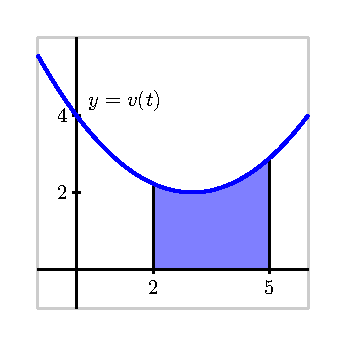
\includegraphics{figures/4_2_Act2Soln.eps}
	\end{center}
	\item $L_4 = \frac{311}{48} \approx 6.47917$, 
	        $R_4 = \frac{335}{48} \approx 6.97917$, and 
	        $M_4 = \frac{637}{96} \approx 6.63542$.
	\item The average of $L_4$ and $R_4$ is
	$$\frac{L_4 + M_4}{2} = \frac{311+335}{96} = \frac{646}{96} \ne \frac{637}{96} = M_4.$$
	This average actually measures what would result from using four trapezoids, rather than rectangles, to estimate the area on each subinterval.  One reason this is so is because the area of a trapezoid is the average of the bases times the width, and the ``bases'' are given by the function values at the left and right endpoints.
	\item If $f$ is positive and increasing on $[a,b]$, $L_n$ will under-estimate the exact area under $f$ on $[a,b]$.  Because $f$ is increasing, its value at the left endpoint of any subinterval will be lower than every other function value in the interval, and thus the rectangle with that height lies exclusively below the curve.  In a similar way, $R_n$ over-estimates the exact area under $f$ on $[a,b]$.
\ea
\end{activitySolution}
\aftera